\chapter{Konzeptuelle Lösung} 
\label{chapter:Kapitel5}
\lhead{Kapitel 5. \emph{Konzeptuelle Lösung}}  
Das Ziel dieser Arbeit ist die Entwicklung eines leichtgewichtigen Prototypen einer Personal Learning Environment auf Basis aktueller Technologien, welcher die Anforderungen aus Kapitel \ref{chapter:Kapitel3} erfüllt. Der Name des entwickelten Systems lautet \emph{Plesynd} (Personal-Learning-Environment Synchronize Data) und wird wie das englische "`pleasant"' (angenehm) ausgesprochen. Plesynd ist ein webbasiertes Dashboard, welches die Möglichkeit bietet mit unterschiedlichen Widgets in Kommunikation zu treten. Wichtig ist hierbei eine Abgrenzung zu zentralisierten Lern-Management-Systemen wie Moodle oder Sakai. Die sind sehr kurszentriert und entsprechen nicht dem nutzerzentrierten Ansatz von Personal Learning Environments. Aus diesem Grund orientiert sich Plesynd viel stärker an bestehenden Widget-Aggregatoren wie iGoogle oder Netvibes (siehe Abschnitt \ref{section:aehnliche_systeme}). In einem nutzerzentrierten Ansatz, muss dem Anwender die Möglichkeit gegeben werden in unterschiedlichen Kontexten mit dem System zu arbeiten. Hierzu erlaubt es Plesynd dem Anwender seine Widgets in einer frei wählbaren Anzahl unterschiedlicher Bereiche, sogenannter Workspaces, aufzuteilen. Der entscheidende Unterschied von Plesynd zu den erwähnten Systemen ist die Offline-Fähigkeit der PLE. Es wurde ein Ansatz entwickelt, der es ermöglicht das System auch ohne Internetverbindung zu starten und Widgets so zu implementieren, dass ihre Informationen offline verfügbar gemacht werden und offline mit Plesynd und den Widgets weitergearbeitet werden kann. Sobald der Browser wieder eine Online-Verbindung hergestellt hat, werden die veränderten Daten mit dem Backend synchronisiert. Zusätzlich zu dem Grundsystem von Plesynd wurde in dieser Arbeit ein Todo-Listen Widget entwickelt, welches die erwähnten Funktionalitäten nutzt und zeigt wie dem System zusätzliche Widgets hinzugefügt und komplett in Plesynd integriert werden können.

Das vorliegende Kapitel liefert einen Überblick über die grundsätzliche Architektur von Plesynd und seiner Komponenten und eine Beschreibung des implementierten User-Interfaces.

\section{Überblick über die Architektur von Plesynd}\label{section:plesynd_architektur}
Abbildung \ref{fig:ueberblick_plesynd_komponenten} gibt einen Überblick über die wichtigsten Komponenten des entwickelten Systems und über deren Zusammenspiel. Plesynd selbst besteht aus zwei Komponenten, Plesynd-Client und Plesynd-Server. Diese liefern zusammen die Funktionalitäten, welche die gestellten Anforderungen erfüllen sollen. Zusätzlich wird Wookie als externe Komponente zum Ausliefern und Erstellen der Widgets verwendet.

\begin{landscape}
\begin{figure}
  \centering
  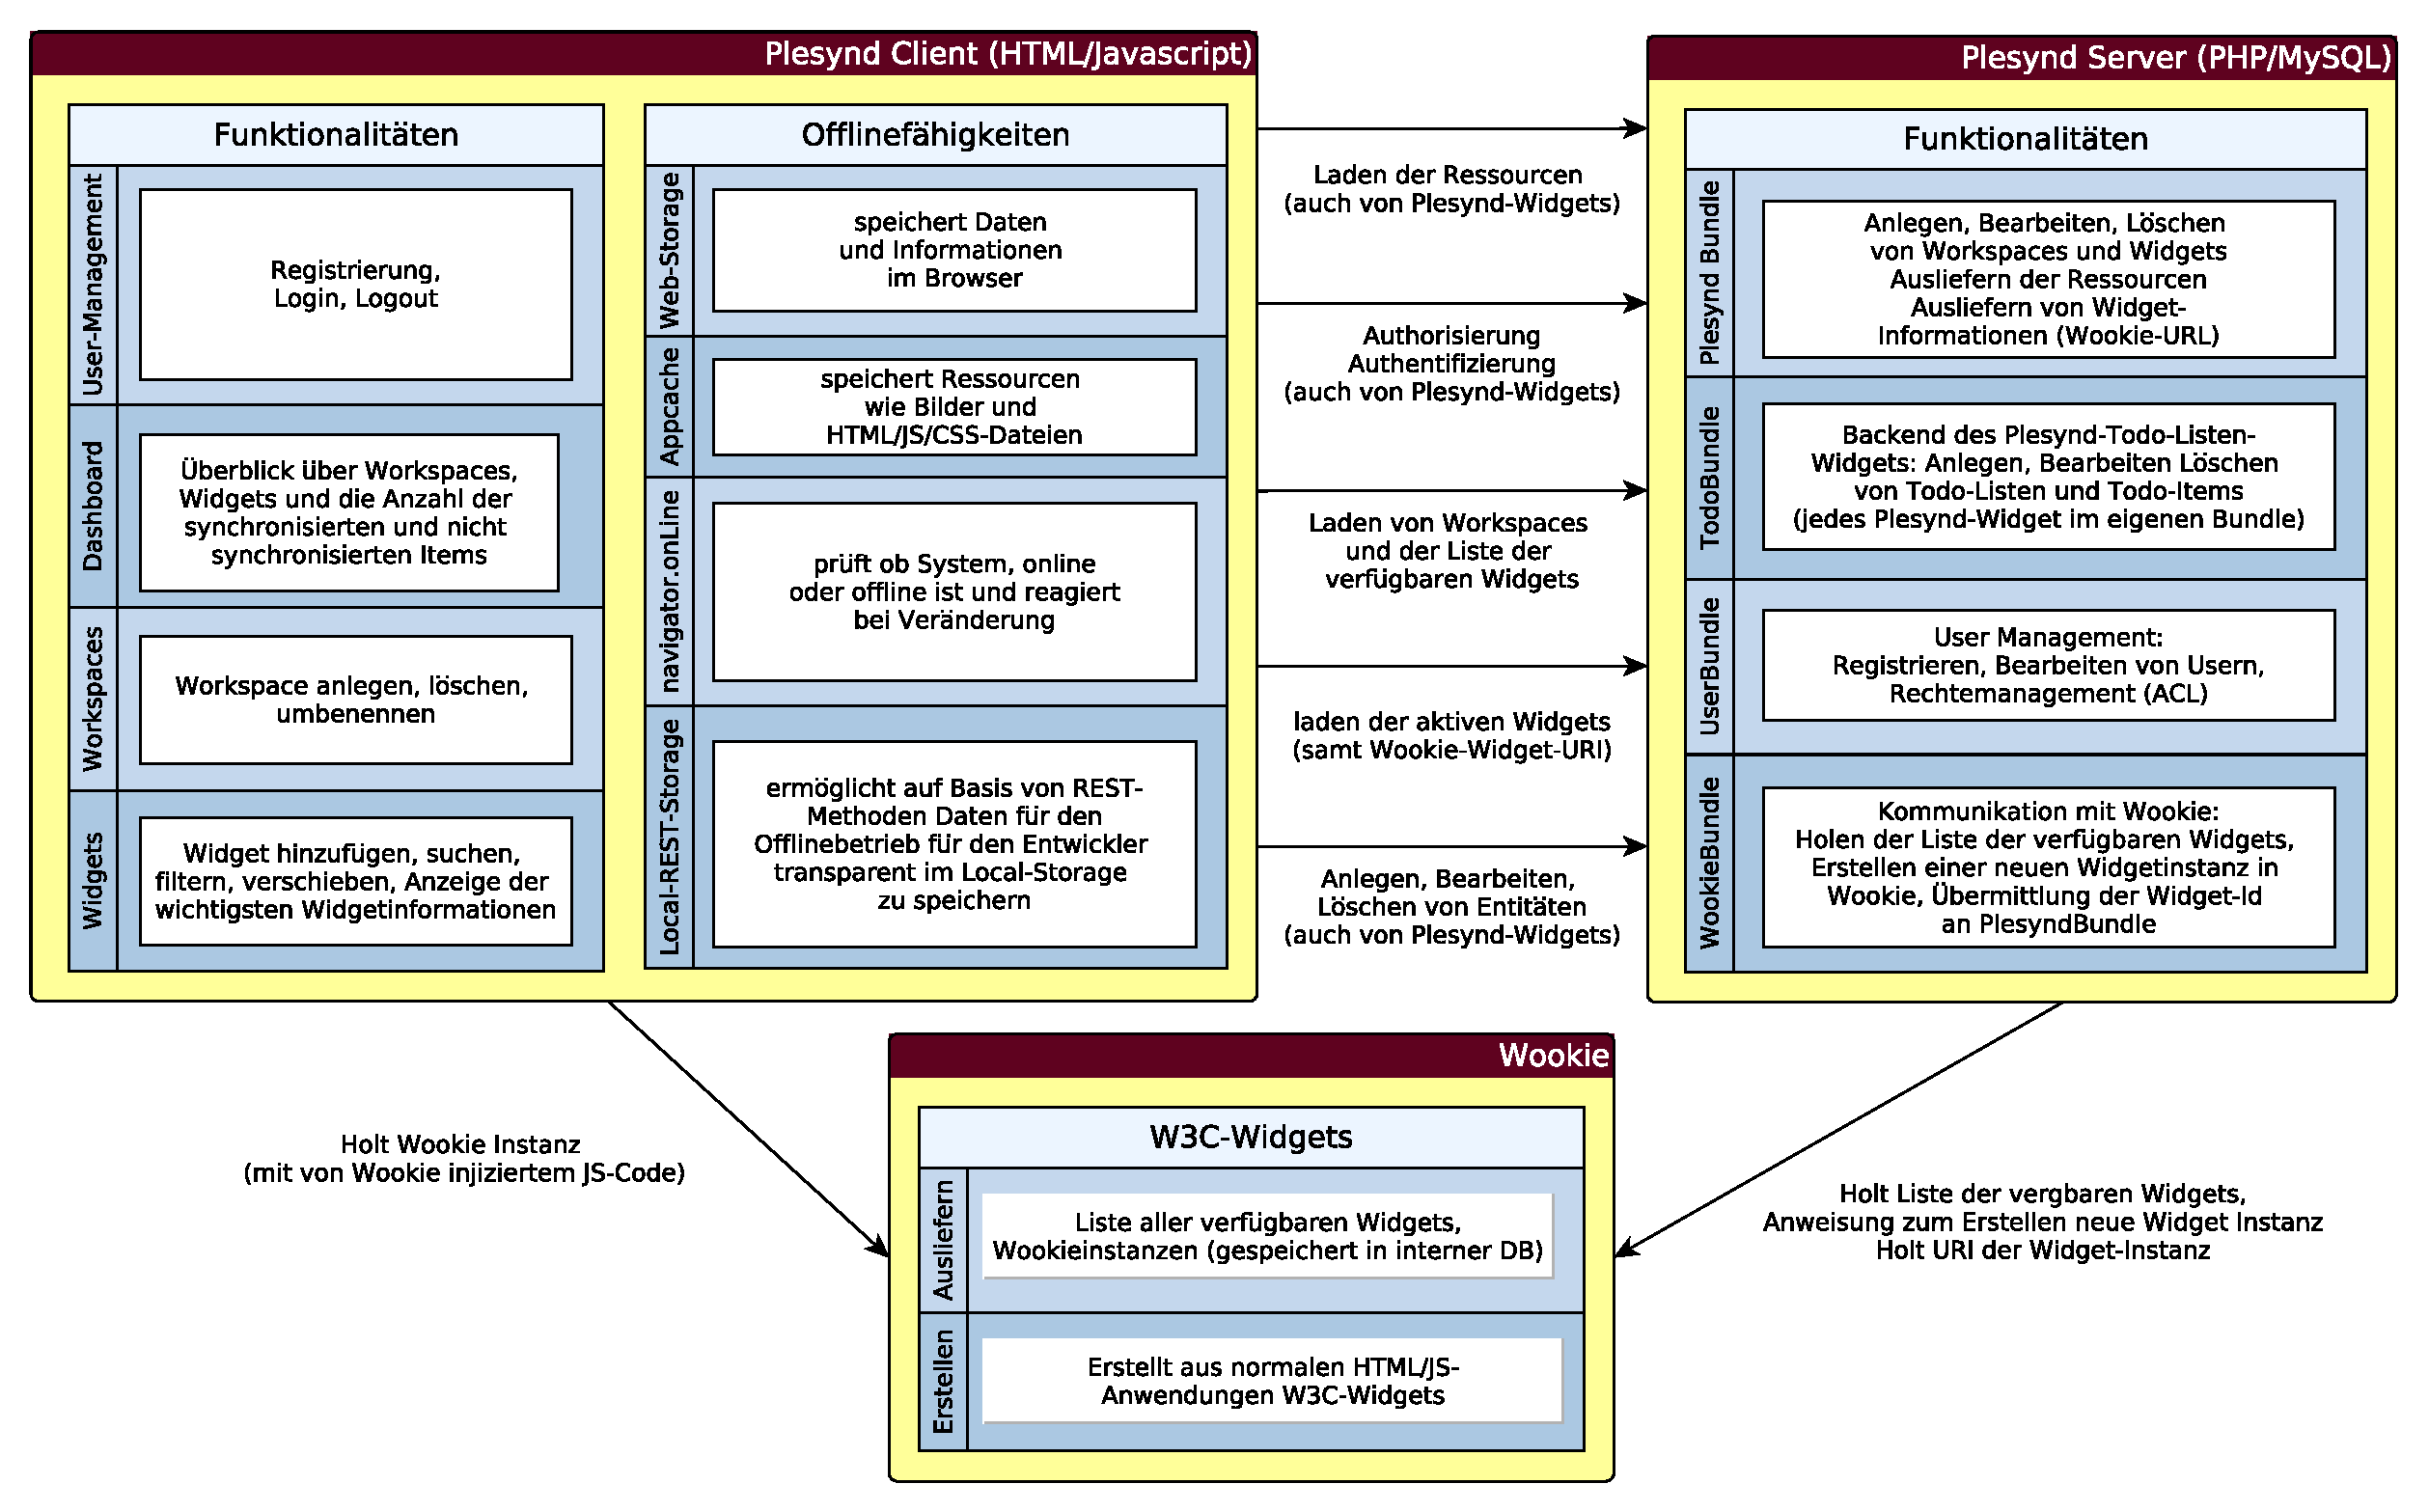
\includegraphics[height=\textheight,keepaspectratio]{./Figures/konzeptionelle_loesung_table.pdf}
    \rule{35em}{0.5pt}
  \caption[Überblick über die Komponenten von Plesynd]{Überblick über die Komponenten von Plesynd}
  \label{fig:ueberblick_plesynd_komponenten}
\end{figure}
\end{landscape}

\subsection{Plesynd-Client}
Plesynd-Client bezeichnet den Teil der Anwendung, der direkt beim Client, also im Browser des Anwenders läuft. Diese Komponente umfasst den größten Teil des entwickelten Systems und ist auch für die Offline-Funktionalitäten von Plesynd verantwortlich. Plesynd-Client stellt über ein User-Interface den Teil der PLE dar, mit dem der Anwender direkt in Berührung kommt. Es liefert Funktionalitäten zum Anlegen und Bearbeiten von Workspaces, versetzt den Anwender in die Lage nach Widgets zu filtern, diese den Workspaces hinzuzufügen und neu anzuordnen und stellt ihm ein Dashboard zur Verfügung auf dem die wichtigsten Informationen zu seinen Workspaces und Widgets zusammengefasst werden. Es informiert den Nutzer auch darüber, ob das System eine Verbindung zu dem Internet hat oder nicht. Zusätzlich gibt es dem Anwender die Möglichkeit sich zu registrieren und in das System einzuloggen. 

Die Fähigkeit von Plesynd und des Todo-Listen-Widgets Anwendungsdaten offline vorzuhalten wurde auf Basis der Web-Storage Technologie entwickelt (siehe \ref{section:offline_storage}). Plesynd erkennt über ein globales Javascript-Event (siehe \ref{section:online_offline_erkennung}), wenn sich der Browser in einem Zustand befindet, in dem er keine Konnektivität mit dem Internet besitzt. Das System informiert den Anwender darüber, kann aber auch entscheiden, welche Funktionalitäten es dem Nutzer nur noch eingeschränkt zur Verfügung stellt. Nimmt der Anwender Änderungen an den Daten vor, werden diese nur in den Local-Storage geschrieben. Sobald sich das System wieder mit dem Internet verbindet, erkennt Plesynd diese Zustandsänderung und synchronisiert die Daten mit den zugrunde liegenden Services. Sollte einmal eine andere Speichertechnik als der Web-Storage benötigt werden, ist das System so implementiert, dass die Art der lokalen Speicherung losgelöst von der restlichen Anwendung umgestaltet werden kann. Entwickelt wurde diese Funktionalität mit besonderem Augenmerk auf die Implementierung zusätzlicher Widgets. Dies bedeutet, dass auf Basis der vorliegenden Implementierung mit relativ wenig Aufwand weitere Widgets für unterschiedliche Services erstellt werden können. Die Art des Services nicht von Belang. Er sollte nur in der Lage ist einfache REST-Anfragen (siehe Abschnitt \ref{section:rest}) zu verstehen, zu verarbeiten und standardkonform auf sie zu antworten. Die Möglichkeit Ressourcen wie Javascript, CSS und HTML Dateien im Browser zu speichern wurde mit der HTML5 Appcache-API umgesetzt (siehe Abschnitt \ref{section:appcache}). Probleme mit der bei modernen Browser üblichen Same-Origin-Policy (siehe \ref{section:same_origin_policy}) für Requests wurden mit dem Cross-Origin Resource Sharing (CORS) Mechanismus und der Postmessage-API gelöst. 

\subsection{Plesynd-Server}
Plesynd-Client ist wie eben beschrieben in der Lage sowohl Ressourcen als auch Daten lokal beim Client zu speichern und so auch offline verfügbar zu machen. Es benötigt zum normalen Betrieb aber ein Backend, welches diese Ressourcen initial ausliefert und sich um die persistente Speicherung der Daten und das Rechtemanagement kümmert. Für diesen Zweck wurde die Plesynd-Server Komponente entworfen. Diese Komponente besteht aus mehreren Bundles (siehe \ref{section:symfony2}), wobei jedes Bundle für einen bestimmten Aufgabenbereich innerhalb  von Plesynd-Server zuständig ist. Aufgaben von Plesynd-Server sind das Ausliefern der Ressourcen, die Speicherung von Workspace und den zugehörigen Widgets samt ihrer Position auf dem Workspaces, das User-Management (Registrierung, Login etc) und das Rechtemanagement, also die Prüfung welcher Nutzer Zugriff auf welchen Workspace, Widget oder welche Todo-Liste hat. 

Plesynd-Server nimmt für die Arbeit mit den Anwendungsdaten (Workspace, Widgets, Todo-Listen etc.) REST konforme Anfragen (siehe \ref{section:rest}) entgegen und antwortet standardkonform.

Für die Abfrage welche Widgets grundsätzlich im System vorhanden sind verwendet Plesynd-Server eine Schnittstelle zur Wookie-Komponente. Diese Schnittstelle wird auch verwendet wenn der Anwender ein neues Widget zu einem Workspace hinzufügen möchten, also eine neue Widget-Instanz erstellt werden muss.

\subsection{Wookie}\label{section:loesung_wookie}
Als externe Komponente wird der W3C-Widget-Container Wookie (siehe \ref{section:widget_frameworks}) eingebunden. Dieser speichert die verfügbaren Widgets in einer internen Datenbank und kann Plesynd so eine Liste der auslieferbaren Widgets zur Verfügung stellen. Wookie hinterlegt außerdem jede einzelne erstellte Widget-Instanz samt ihrem Zustand und kann so das eigentliche Widget bei Bedarf an Plesynd-Client ausliefern. Diese Funktionalität ist die einzige, bei der Plesynd-Client direkt Kontakt zu Wookie aufnimmt, ansonsten wird die gesamte Kommunikation über Plesynd-Server abgewickelt. Zusätzlich zu diesen Anwendungsfällen bietet Wookie Werkzeuge an, um aus normalen HTML/Javascript-Applikationen ein W3C-Widget zu erstellen. Diese Funktionalität steht jedoch nicht über die Kommunikation mit Plesynd zur Verfügung, sondern muss über die Kommandozeile in Anspruch genommen werden.

\section{User Interface}\label{section:user_interface}
\begin{figure}
  \centering
  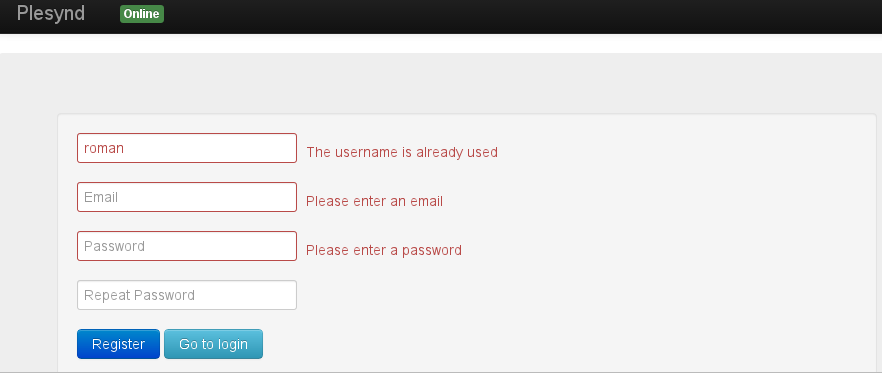
\includegraphics[width=\textwidth,height=\textheight,keepaspectratio]{./Figures/plesynd_register.png}
    \rule{35em}{0.5pt}
  \caption[Plesynd User-Interface: Registrieren]{Der Anwender kann sich für die Nutzung von Plesynd registrieren}
  \label{fig:plesynd_register}
\end{figure}

Für die Umsetzung der Screen-Dimension (siehe Abschnitt \ref{section:dimensions_palmer}), also des User-Interfaces kommen in Plesynd drei wichtige Konzepte zum Einsatz: Dashboard, Widgets und Workspaces. Über Widgets werden die unterschiedlichen Werkzeuge und Services, die ein Nutzer innerhalb des Systems nutzen möchte eingebunden (siehe: Abschnitt \ref{section:widgets}). Die Umsetzung der einzelnen Widgets liegt in der Hand des jeweiligen Designers. Das Ziel beim Design von Plesynd war es dem Nutzer die Bedienung so einfach wie möglich zu machen. Die wichtigsten Informationen sollten ihm direkt direkt zur Verfügung gestellt werden (sind alle Daten aktuell, welche Widgets werden benutzt, ist das System offline oder online etc). Widgets können gesucht, nach Offline-Kompatibilität gefiltert und dem System hinzugefügt werden. Es existiert ein Dashboard (siehe Abbildung \ref{fig:plesynd_dashboard}), welches dem Nutzer anzeigt welche Widgets auf welchen Workspaces zur Verfügung stehen und wie ihr Online-/Offline-Status ist.
\begin{figure}
  \centering
  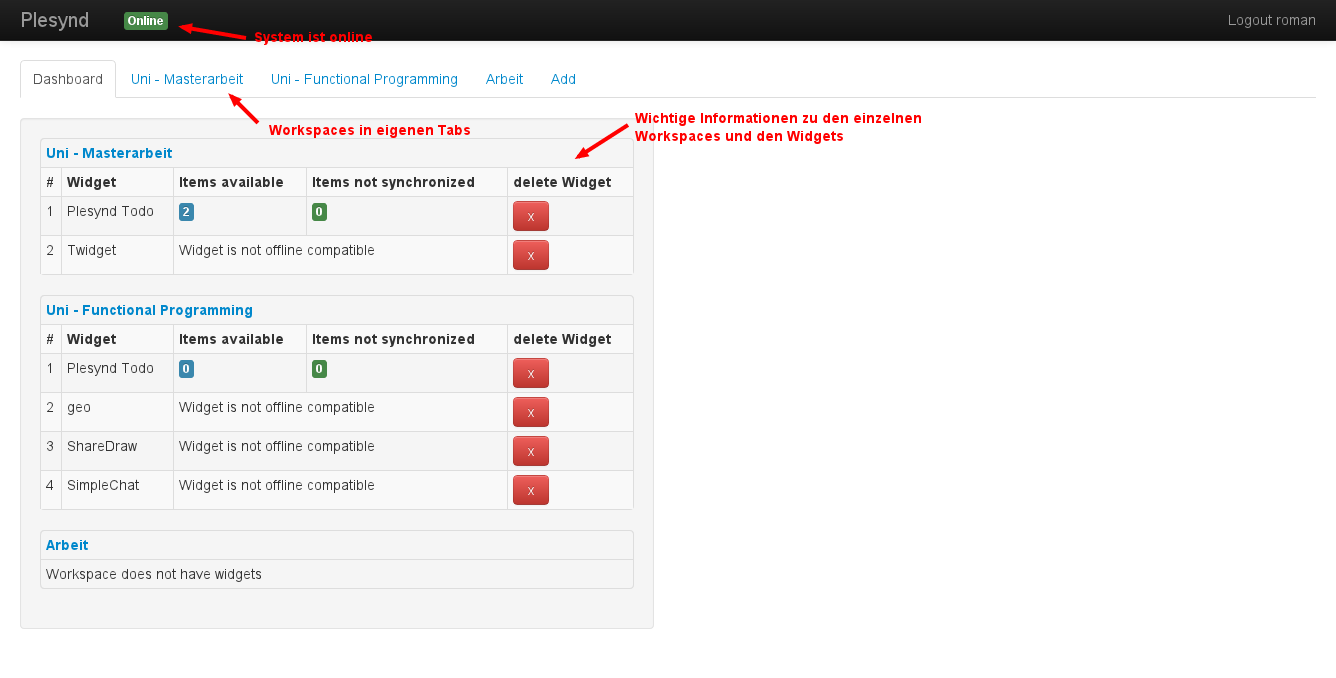
\includegraphics[width=\textwidth,height=\textheight,keepaspectratio]{./Figures/plesynd_dashboard.png}
    \rule{35em}{0.5pt}
  \caption[Plesynd User-Interface: Dashboard]{Das Dashboard fasst die wichtigsten Informationen zusammen.}
  \label{fig:plesynd_dashboard}
\end{figure}

Da Plesynd Wookie als Widget Container benutzt, ist es möglich alle W3C-Widgets in das System einzubinden. Für diese Arbeit wurde ein Todo-Listen-Service entwickelt für den als prototypische Entwicklung ein Widget mit Online-/Offline-Fähigkeiten implementiert wurde. Besitzt ein Widget Online-/Offline-Fähigkeiten so erhält es eine von Plesynd zur Verfügung gestellte Statusleiste, in der der aktuelle Online-/Offline-Status, sowie die Anzahl der verfügbaren Einträge und der noch nicht synchronisierten Einträge angezeigt wird (siehe Abbildungen \ref{fig:plesynd_workspace_online} und \ref{fig:plesynd_workspace_offline}).
\begin{figure}
  \centering
  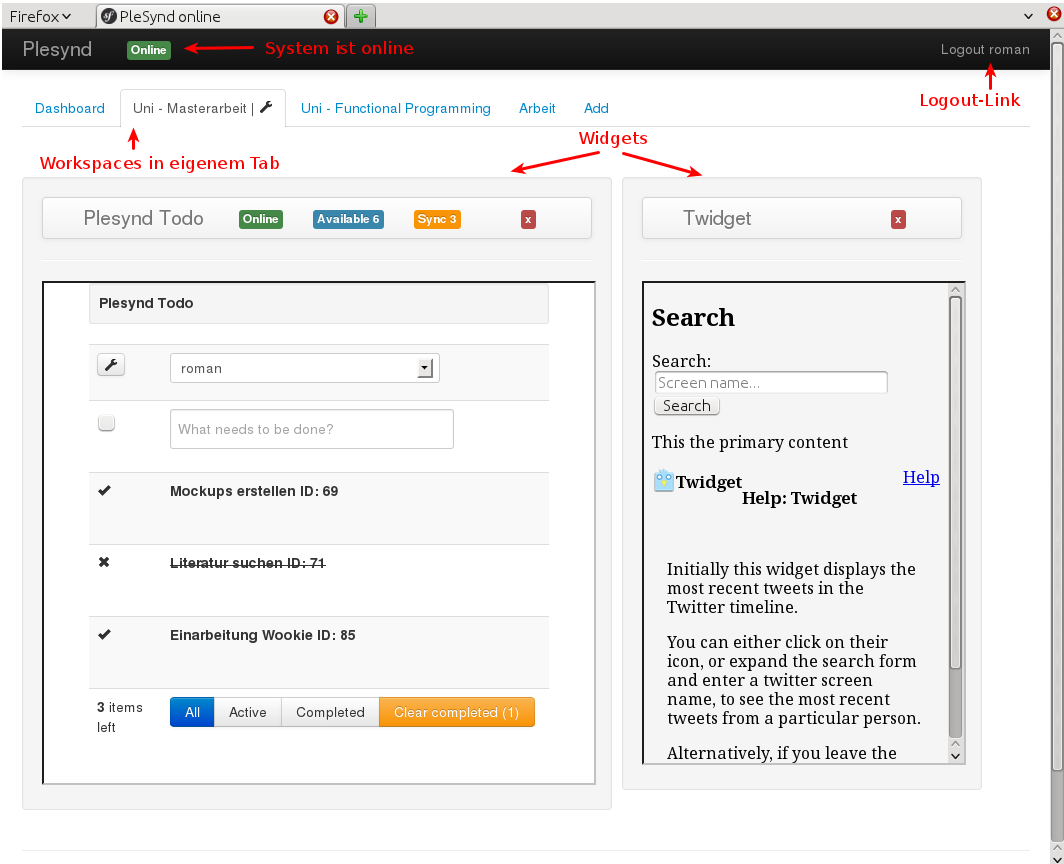
\includegraphics[width=\textwidth,height=\textheight,keepaspectratio]{./Figures/plesynd_workspace_online.png}
    \rule{35em}{0.5pt}
  \caption[Plesynd User-Interface: Workspace Online]{Ein Workspace mit unterschiedlichen Widgets}
  \label{fig:plesynd_workspace_online}
\end{figure}

\begin{figure}
  \centering
  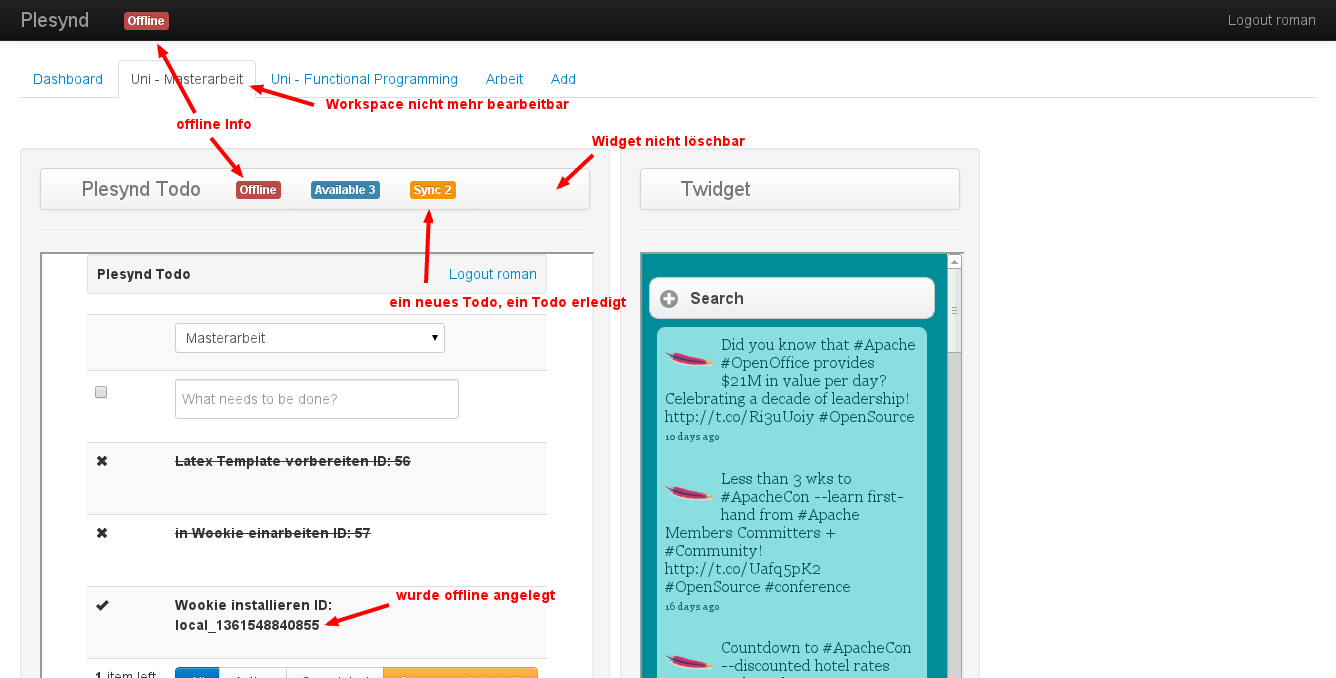
\includegraphics[width=\textwidth,height=\textheight,keepaspectratio]{./Figures/plesynd_workspace_offline.png}
    \rule{35em}{0.5pt}
  \caption[Plesynd User-Interface: Workspace Offline]{Die wichtigsten Unterschiede im Offline-Modus}
  \label{fig:plesynd_workspace_offline}
\end{figure}
Der Nutzer hat die Möglichkeit Widgets nach Themen oder Einsatzgebieten zu gruppieren. Dies geschieht über sogenannte Workspaces. Workspaces sind vom Nutzer frei und in unbegrenzter Zahl hinzufügbare Bereiche im System. Sie sind über eine Reiter-Navigation zu erreichen und können jederzeit umbenannt oder auch wieder gelöscht werden (siehe Abbildung \ref{fig:plesynd_workspace_edit}). 
\begin{figure}
  \centering
  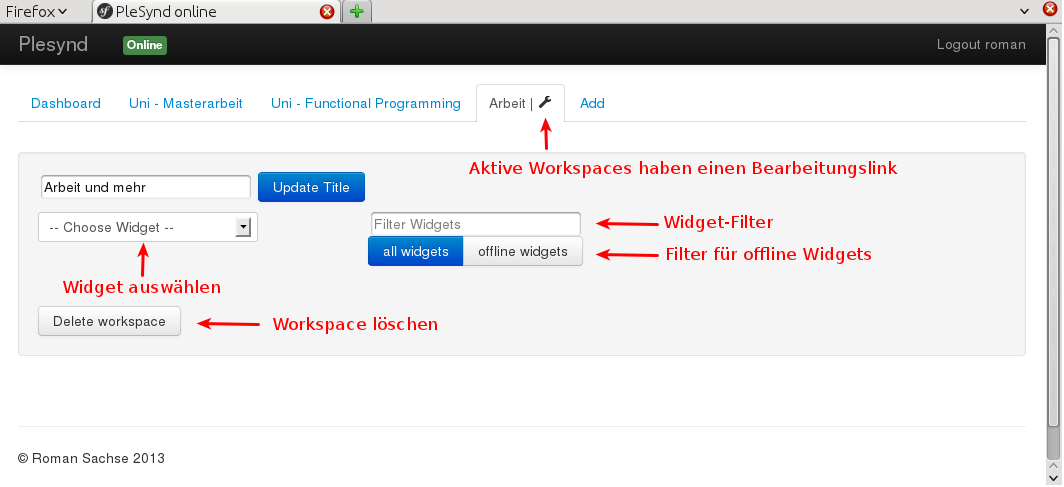
\includegraphics[width=\textwidth,height=\textheight,keepaspectratio]{./Figures/plesynd_workspace_edit.png}
    \rule{35em}{0.5pt}
  \caption[Plesynd User-Interface: Bearbeiten von Workspaces]{Workspaces können direkt bearbeitet werden.}
  \label{fig:plesynd_workspace_edit}
\end{figure}
Jedes Widget kann einem Workspace hinzugefügt werden. Die Position der Widgets innerhalb eines Workspaces kann über einen Drag and Drop Mechanismus angepasst werden. Die Startseite stellt als Dashboard die wichtigsten Informationen dar. Jeder Workspace wird in einer eigenen Tabelle inklusive seiner Widgets und der Anzahl der zur Verfügung stehenden Widgets präsentiert. Über direkte Links innerhalb des Dashboards ist es dem Nutzer möglich direkt zu dem gewünschten Workspace zu navigieren (siehe Abbildung \ref{fig:plesynd_dashboard}).
